\documentclass{article}
\usepackage[preprint]{neurips}
\usepackage[utf8]{inputenc}
\usepackage[T1]{fontenc}
\usepackage[hidelinks]{hyperref}
\usepackage{url}
\usepackage{booktabs}
\usepackage{amsfonts}
\usepackage{amsmath}
%\usepackage{nicefrac}
%\usepackage{microtype}
\usepackage{xcolor}
\usepackage{graphicx}
\usepackage{subcaption}
\usepackage{enumitem}
\usepackage{multirow}
\usepackage{algorithm}
\usepackage{algorithmic}

\definecolor{bestcolor}{HTML}{006400}

\title{CER-Bench: A Constrained Evidence Retrieval Benchmark\\ for Biomedical Literature}

\author{
  Anonymous Authors\\
  NeurIPS 2026 Evaluations \& Datasets Track
}

\begin{document}
\maketitle

% ============================================================================
\begin{abstract}
We introduce \textsc{CER-Bench}, a benchmark of 304~tasks across eight retrieval families for condition-sensitive evidence collection in biomedical literature. Existing scientific retrieval benchmarks predominantly reward topical matching, yet real scientific search requires satisfying structured experimental constraints, reconciling condition-dependent contradictions, tracking consensus evolution over time, aggregating quantitative evidence across studies, and knowing when to abstain. Our benchmark tests all of these through eight task families---constraint-satisfaction, comparative, contradiction, abstention, multi-hop, temporal, aggregation, and negative-result retrieval---each grounded in real documents from a 4,936-paper corpus spanning ten biomedical subdomains. We evaluate eleven retrieval configurations spanning lexical (BM25), dense (SPECTER2, BGE, E5-large, MedCPT), learned sparse (SPLADE), hybrid fusion, reranking (ms-marco, BGE-reranker), and iterative agentic search, alongside two purpose-trained controllers (Qwen3-8B and gpt-oss-20b fine-tuned on teacher traces). \textbf{Our central finding is that no single method dominates: CER-Bench is diagnostic, exposing distinct regimes rather than crowning a winner.} On the v1 split (2--3 seeded gold per task), BM25 leads on MRR, SPLADE is the strongest single-pass retriever (highest R@5 and R@10 among non-agentic methods), and an iterative agent achieves the highest deeper recall (R@20). \emph{Both stronger-label evaluations reverse this aggregate ordering}: on a cluster-first v2 split (9.8 gold/task) BM25 leads on every aggregate metric, and on LLM-judge pooled adjudication (12.7 gold/task) BGE leads on R@20 with the agent dropping to fifth. The agent retains family advantages on temporal and comparative tasks across both stronger-label regimes. Family-aligned structured metrics tell a similar story: the agent's clearest advantage is \emph{complete-collection rate} on aggregation (29.4\% vs.\ 5.9\% for BM25). An ablation isolating iterative refinement shows it accounts for the agent's recall gains: restricting the controller to a single search round reduces Recall@10 by 14.4~points. Abstention---recognizing when the corpus lacks sufficient evidence---remains completely unsolved by all methods. Aggregate significance claims should be read as v1-specific; results vary under expanded gold labels (no multiple-comparison correction is applied). We release the benchmark, corpus, baselines, trained controllers, and evaluation code, with Croissant metadata and RAI documentation, to support future work on scientific evidence retrieval.
\end{abstract}

% ============================================================================
\section{Introduction}
\label{sec:intro}

Scientific literature retrieval is harder than general web search. A working scientist does not type a keyword and scroll through ten blue links; instead, they ask questions that involve multiple experimental constraints (``find CRISPR studies in human iPSC-derived cardiomyocytes targeting ion channel mutations''), require evidence from both sides of a comparison (``compare transfection efficiency of lipofection vs.\ electroporation in primary T~cells''), or demand reconciliation of apparently contradictory findings that turn out to be conditional on cell type, dosage, or organism. Existing retrieval benchmarks---designed around single-answer, keyword-friendly queries---do not evaluate these capabilities.

Recent work has highlighted this gap from multiple angles. DORIS-MAE~\cite{dorismae2023} demonstrated substantial performance drops for seventeen retrieval methods on complex scientific queries. LitSearch~\cite{litsearch2024} showed that dense retrieval can improve over BM25 by 24.8 absolute Recall@5 points on realistic literature-search queries, but its tasks remain single-turn and answer-focused. EpiBench~\cite{epibench2026} pushes toward multi-turn multimodal research workflows but reports only 29.2\% hard-split accuracy for the strongest model, and its broad scope dilutes depth in any one domain.

On the systems side, OpenScholar~\cite{openscholar2026} showed that a retrieval-augmented 8B model over 45 million open-access papers can outperform GPT-4o on scientific question answering, and PaperQA2~\cite{skarlinski2024paperqa2} demonstrated strong end-to-end literature synthesis. Context-1~\cite{context2026} introduced a self-editing retrieval agent trained on over 8,000 synthetic tasks, showing that a cheap four-rollout configuration with reciprocal-rank fusion can match much larger frontier models. Yet none of these systems have been evaluated on condition-sensitive, multi-constraint scientific retrieval tasks, and no benchmark exists that systematically tests these capabilities.

Figure~\ref{fig:taxonomy} provides an overview of the eight task families. We contribute:
\begin{itemize}[leftmargin=*,itemsep=2pt,topsep=2pt]
\item \textbf{A benchmark} of 304 corpus-grounded tasks across \textbf{eight retrieval families}---constraint-satisfaction, comparative, contradiction, abstention, multi-hop, temporal, aggregation, and negative-result retrieval---each testing a distinct evidence-collection capability that single-query retrieval struggles with.
\item \textbf{A biomedical corpus} of 4,936 documents (17,902 chunks) from PubMed Central Open Access, enriched with MeSH terms, citation graphs from OpenAlex, and scientific-structure chunking.
\item \textbf{Comprehensive baselines}: eleven retrieval configurations spanning lexical (BM25), learned sparse (SPLADE), four dense models, hybrid fusion, two rerankers, and a reference iterative controller, with paired bootstrap significance tests, family-aligned structured metrics, and a simple abstention threshold baseline.
\item \textbf{Key findings (diagnostic, not promotional)}: (1)~no single method dominates across families or label regimes---BM25 leads on MRR and on the stronger-label v2 split, SPLADE on single-pass recall (highest R@5/R@10 among non-agentic methods), and iterative search on v1 R@20; (2)~reranking with general-purpose cross-encoders degrades scientific retrieval; (3)~dense retrieval quality depends on the embedding model, not the paradigm; (4)~the agent's clearest structural advantage is \emph{complete-collection} on aggregation tasks (29.4\% vs.\ 5.9\% BM25); and (5)~abstention remains an open problem (AUROC~0.714 for a simple threshold baseline). We frame CER-Bench as a tool for surfacing these regime differences rather than promoting any single retriever.
\item \textbf{Gold-label robustness}: we report two complementary validations---LLM-judge pooled adjudication (gold expanded from 2.4 to 12.7 docs/task across all methods' top-20) and a parallel cluster-first v2 split (9.8 gold/task by construction)---and disclose a 30-task human-validation protocol whose results will appear in the camera-ready (Appendix~\ref{app:humanpilot}). Method ordering shifts under stronger labels, which we surface in the main results.
\end{itemize}

\begin{figure}[t]
\centering
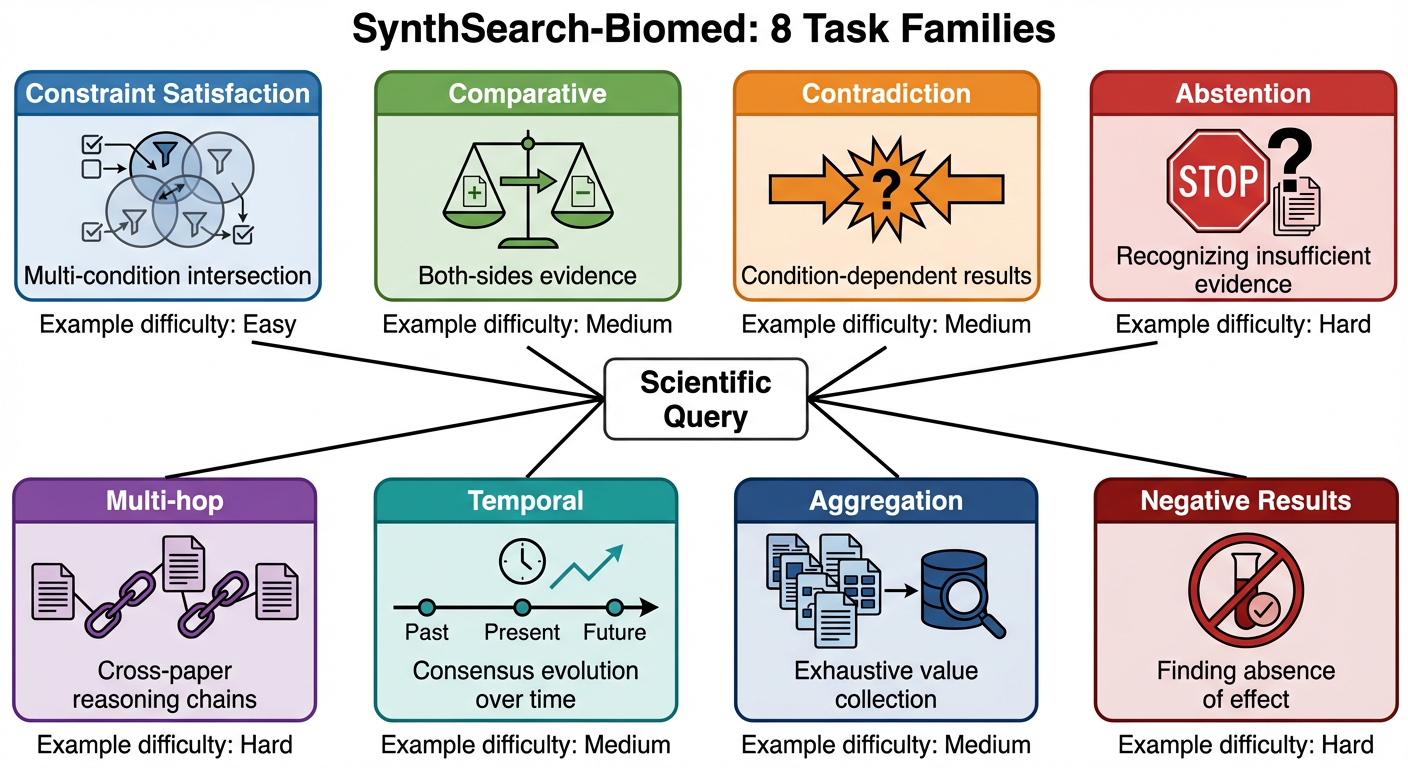
\includegraphics[width=\textwidth]{figures/task_taxonomy.png}
\caption{Overview of the eight task families in \textsc{CER-Bench}. Each family tests a distinct retrieval capability needed for real scientific workflows. Families range from constraint-satisfaction (intersection of experimental conditions) to abstention (recognizing when the corpus cannot support a query). All families are balanced at 38 tasks each.}
\label{fig:taxonomy}
\end{figure}

% ============================================================================
\section{Related Work}
\label{sec:related}

\paragraph{Scientific retrieval systems.}
SPECTER2~\cite{specter2} provides scientific document embeddings trained across 23 fields of study with task-specific adapters for retrieval, classification, and recommendation. OpenScholar~\cite{openscholar2026} combines retrieval over 45M papers with an 8B language model to achieve state-of-the-art scientific question answering. PaperQA2~\cite{skarlinski2024paperqa2} builds an end-to-end pipeline for literature synthesis. These systems focus on answer generation; our work evaluates the retrieval step in isolation, which is where most evidence-collection failures originate.

\paragraph{Retrieval agents.}
Context-1~\cite{context2026} introduced a 20B self-editing search agent trained on 8,000+ synthetic tasks. Its decompose--search--prune--refine loop motivates our iterative controller, but we use only a prompt-based BM25 search loop rather than a trained policy, reciprocal-rank fusion, or learned pruning. This keeps the method reproducible while isolating iterative query refinement from model-specific training infrastructure.

\paragraph{Scientific retrieval benchmarks.}
Established biomedical IR benchmarks include BioASQ~\cite{bioasq2015} (semantic indexing and QA), TREC Precision Medicine~\cite{trecpm2017} (clinical trial matching), and SciFact~\cite{scifact2020} (claim verification). BEIR~\cite{beir2021} provides heterogeneous zero-shot evaluation across domains. DORIS-MAE~\cite{dorismae2023} evaluates retrieval on complex scientific queries. LitSearch~\cite{litsearch2024} tests realistic literature-search queries. ScholarQABench, introduced with OpenScholar~\cite{openscholar2026}, evaluates scientific answer correctness. EpiBench~\cite{epibench2026} benchmarks multi-turn multimodal workflows. Our benchmark complements these by (i)~testing eight distinct retrieval \emph{families} rather than a single task type, (ii)~grounding all tasks in actual corpus documents, (iii)~including explicit abstention evaluation, and (iv)~focusing on evidence \emph{retrieval} rather than end-to-end answer generation.

\paragraph{Hybrid, fusion, and iterative retrieval.}
Reciprocal rank fusion (RRF)~\cite{rrf2009} combines ranked lists without score calibration. Recent iterative full-paper retrieval work explores multi-aspect expansion with post-order aggregation~\cite{cor2025}, motivating our controller at a high level while leaving RRF and learned pruning out of our implementation. BERT-style cross-encoder rerankers~\cite{nogueira2019bert} often improve precision in web passage retrieval, but the web-trained rerankers we tested degrade scientific retrieval on our benchmark. Classical PRF (RM3, Rocchio)~\cite{robertson2009} and learned expansion (DocT5Query, SPLADE~\cite{splade2022}) address query refinement via term reweighting; we evaluate BM25+RM3 and find it does not improve over BM25.

% ============================================================================
\section{CER-Bench}
\label{sec:benchmark}

\subsection{Corpus}

We construct a biomedical literature corpus from four sources: PubMed (abstracts, MeSH terms, publication metadata)~\cite{pubmed_nlm}, PubMed Central Open Access (full-text XML)~\cite{pmc_nlm}, OpenAlex (citation graph, concepts, topics)~\cite{openalex2022}, and Semantic Scholar/S2ORC metadata (fields of study)~\cite{s2orc2020}. We query ten seed subdomains chosen for their richness in experimental conditions and method comparisons: CRISPR gene editing, immune checkpoint immunotherapy, drug repurposing, CAR-T cell therapy, organoid disease models, single-cell sequencing, gut microbiome, mRNA therapeutics, protein structure prediction, and epigenetics.

After filtering editorials, letters, and comments and restricting to English-language 2015--2026 articles, the corpus contains \textbf{4{,}936 documents}; 652 have PMC full text parsed into structured sections, the remaining 4{,}284 are abstract-only. Scientific-structure chunking (not fixed windows) yields \textbf{17{,}902 chunks} (median 304 tokens, ${\sim}$6.6M tokens), each inheriting its parent's metadata.

\subsection{Task Families}

We define eight retrieval families, each testing a distinct capability that working scientists need but existing benchmarks under-evaluate. Table~\ref{tab:families} summarizes the taxonomy.

\begin{table}[t]
\centering
\caption{Eight task families in \textsc{CER-Bench}, each testing a distinct retrieval capability. All families are balanced at 38 tasks each (304 total).}
\label{tab:families}
\small
\begin{tabular}{lp{5.5cm}l}
\toprule
\textbf{Family} & \textbf{Description} & \textbf{Key Challenge} \\
\midrule
Constraint & Find papers satisfying multiple experimental constraints simultaneously & Intersection over unions \\
Comparative & Retrieve evidence from both sides of a comparison & Balanced both-sides recall \\
Contradiction & Reconcile conflicting findings conditional on experimental setup & Condition tracking \\
Abstention & Recognize when corpus lacks sufficient evidence & Resisting false confidence \\
Multi-hop & Chain evidence across 3+ papers via shared entities & Bridging entity discovery \\
Temporal & Track how findings evolved over time & Time-distributed retrieval \\
Aggregation & Collect all reported values for a measurement & Exhaustive recall \\
Negative & Find papers reporting null or negative findings & Overcoming positive-result bias \\
\bottomrule
\end{tabular}
\end{table}

\paragraph{Constraint-satisfaction} tasks specify 2--4 experimental constraints (organism, assay, intervention, outcome, time period). Only papers satisfying \emph{all} constraints are relevant. Topic matching alone fails because many papers match individual constraints but not their intersection.

\paragraph{Comparative} tasks ask for evidence from both sides of a comparison (e.g., two methods, two organisms). Systems that retrieve only one side receive partial credit.

\paragraph{Contradiction/conditionality} tasks present findings that appear contradictory across papers but are conditional on experimental setup. A contradiction is labeled when two or more gold documents report opposing outcomes (e.g., ``inhibits growth'' vs.\ ``no effect on growth'') for the same intervention, where the discrepancy is explained by a documented difference in conditions (cell type, dosage, organism, assay protocol). The system must retrieve evidence showing both outcomes and the resolving conditions.

\paragraph{Abstention} tasks ask questions that the corpus cannot support. The correct behavior is to recognize this and abstain rather than returning marginally relevant results. Tasks are constructed by combining plausible constraints that no document satisfies jointly.

\paragraph{Multi-hop} tasks require chaining evidence across three or more papers via shared entities (a gene, pathway, compound, or mechanism). No single paper answers the full question.

\paragraph{Temporal} tasks ask how findings or consensus changed over time. The system must retrieve papers from different eras, not just the most recent or most cited.

\paragraph{Aggregation} tasks ask to collect all reported quantitative values for a specific measurement across studies. Exhaustive recall is the key challenge.

\paragraph{Negative-result} tasks ask specifically for studies reporting null findings or absence of effect. A document is labeled as a negative-result gold document if it contains explicit statements of non-significance (e.g., ``no significant difference,'' ``failed to replicate,'' ``did not reach statistical significance'') with respect to the queried intervention-outcome pair. Publication bias toward positive results makes these documents harder to surface.

\subsection{Task Generation}

We use a \textbf{corpus-grounded} generation pipeline to ensure all gold labels correspond to real documents. For each task:
\begin{enumerate}[leftmargin=*,itemsep=1pt,topsep=2pt]
\item \textbf{Sample} 2--3 related papers from the corpus, stratified by seed subdomain.
\item \textbf{Generate} a question using an LLM (Claude Sonnet 4) conditioned on the sampled papers' titles, abstracts, and metadata. The prompt specifies the target family and requires constraints drawn from exact terms in the abstracts.
\item \textbf{Assign gold labels}: the sampled paper IDs become the supporting documents. For abstention tasks, the sampled papers become near-miss hard negatives, and the gold evidence set is empty.
\end{enumerate}

This pipeline produces 304 tasks (38 per family), split into 119 train, 60 dev, and 125 test tasks, stratified by family. Per-family test counts: constraint~15, comparative~15, contradiction~14, abstention~17, multi-hop~16, temporal~17, aggregation~17, negative~14. The test split is locked before evaluation.

% ============================================================================
\section{Iterative Search Controller}
\label{sec:method}

We implement a minimal, prompt-based iterative search controller that searches the corpus, evaluates retrieved evidence, and refines its search query across multiple rounds. The design is inspired by Context-1~\cite{context2026} but deliberately stripped down: we use only lexical search (BM25) as the retrieval tool, with no metadata filtering, citation-graph traversal, or structured entity extraction. This isolates the contribution of \emph{iterative query refinement alone} from other possible enhancements. Figure~\ref{fig:agent} illustrates the architecture.

\begin{figure}[t]
\centering
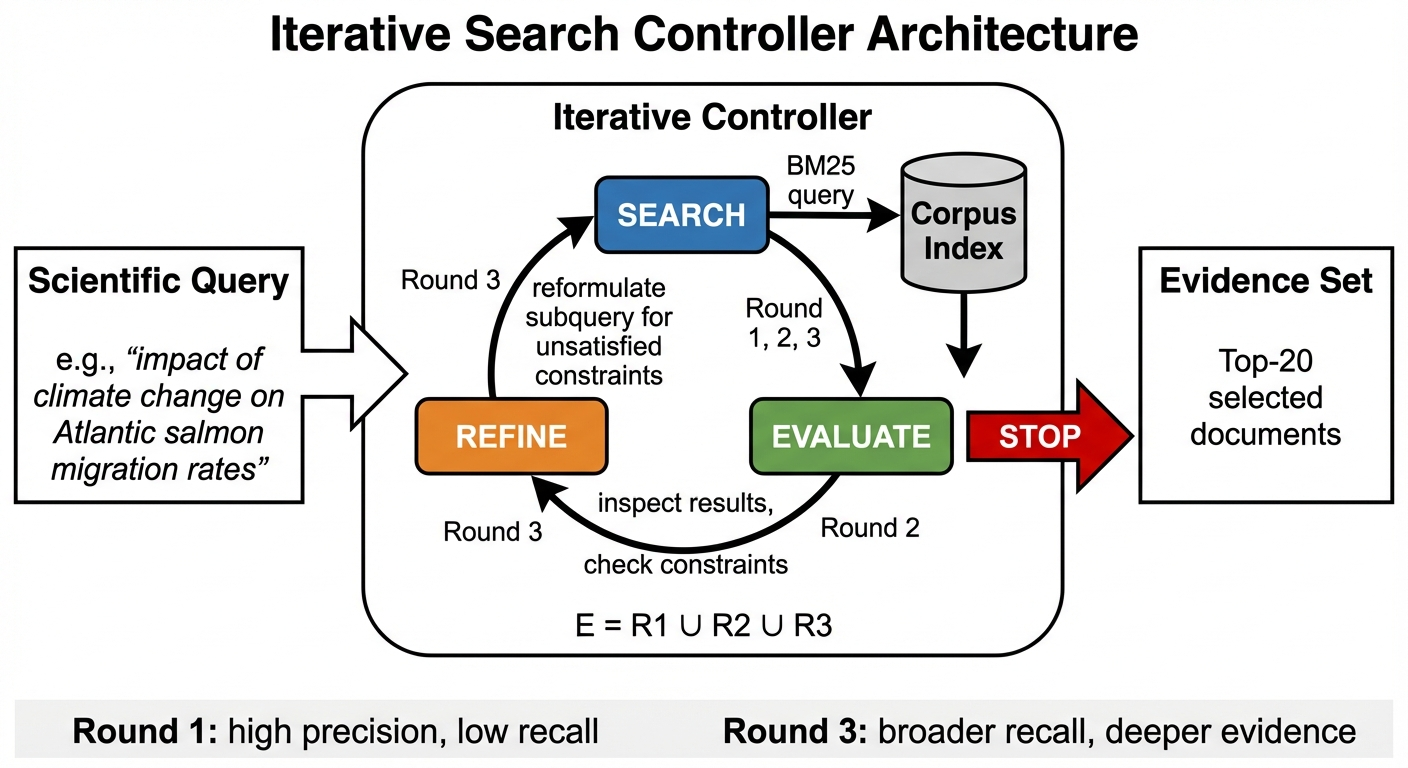
\includegraphics[width=\textwidth]{figures/agent_architecture.png}
\caption{Iterative search controller architecture. The controller executes up to $T{=}3$ rounds of \textsc{Search}$\to$\textsc{Evaluate}$\to$\textsc{Refine}, accumulating evidence across rounds. Each round generates a refined subquery targeting unsatisfied constraints. The cumulative evidence set $E = \bigcup_t R_t$ grows with each round; at termination the controller selects its top-20 documents.}
\label{fig:agent}
\end{figure}

\subsection{Architecture}

The controller operates in a loop of at most $T=3$ rounds. At each round $t$, it selects one of three actions:
\begin{itemize}[leftmargin=*,itemsep=1pt,topsep=2pt]
\item \textsc{Search}$(q_t)$: execute a BM25 query over the chunk index, returning the top-8 chunk results per round with document titles and 120-character text snippets. Retrieved chunks are deduplicated across rounds (chunks seen in prior rounds are excluded).
\item \textsc{Refine}$(q_{t-1}, E_t)$: given the current evidence set $E_t$ and the original question, generate a refined subquery targeting unsatisfied constraints.
\item \textsc{Stop}$(S)$: return the selected document set $S \subseteq E_t$.
\end{itemize}

The controller maintains a cumulative evidence set $E = \bigcup_{t=1}^{T} R_t$ where $R_t$ is the set of unique documents retrieved at round $t$. Termination occurs when: (a)~the controller issues a \textsc{Stop} action, returning an explicit list of document IDs from $E$ (deterministic at temperature~0); or (b)~the maximum round count $T{=}3$ is reached, in which case all documents in $E$ are returned in retrieval order. No score fusion or normalization across rounds is applied. We observe that later rounds occasionally introduce marginally relevant documents that dilute precision (the agent's R@5 is below BM25's), suggesting that dynamic stopping or pruning could improve the precision--recall trade-off. We leave this to future work, noting that Context-1~\cite{context2026} addresses this via a learned pruning policy.

\subsection{Backbone and Prompting}

The controller uses Claude Sonnet 4 as its reasoning backbone. A system prompt defines the three actions and instructs the model to: (1) analyze the question and identify key constraints, (2) search broadly first, (3) evaluate which constraints are satisfied, (4) refine queries for unsatisfied constraints, and (5) stop when evidence is sufficient. The model responds with a JSON action at each round.

This design is deliberately minimal. Unlike Context-1, we do not train a specialized model; the controller is entirely prompt-based. This makes it reproducible with any capable LLM and isolates the contribution of iterative search from model-specific capabilities.

% ============================================================================
\section{Experiments}
\label{sec:experiments}

\subsection{Baselines}

We evaluate eleven retrieval configurations spanning five paradigms:

\textbf{Lexical}: BM25 (Okapi, $k_1{=}1.2$, $b{=}0.75$)~\cite{robertson2009} over 17,902 chunks.

\textbf{Dense}: SPECTER2~\cite{specter2} with proximity adapter (scientific-specific, 768-dim); BGE-base-en-v1.5~\cite{bge2024} (general-purpose, 768-dim); E5-large-v2~\cite{e52022} (general-purpose, 1024-dim); MedCPT~\cite{medcpt2023} (biomedical-specific, separate query/article encoders, 768-dim). All use FAISS inner-product search~\cite{johnson2019faiss}.

\textbf{Learned sparse}: SPLADE~\cite{splade2022} (\texttt{naver/splade-cocondenser-ensembledistil}), a pre-trained learned sparse retriever using MLM logit expansion. We use the public checkpoint without domain adaptation; documents are encoded to sparse vectors (max-pooled log-saturated logits over the vocabulary), indexed with scipy sparse matrices, and scored via dot product.

\textbf{Fusion \& reranking}: Hybrid (RRF of BM25+SPECTER2, $k{=}60$); Hybrid + ms-marco-MiniLM cross-encoder on top-50; BM25 + BGE-reranker-v2-m3 on BM25 top-50. We do not test biomedical-specific rerankers; our negative reranking results are domain-mismatch findings, not general claims about reranking.

\textbf{Iterative agent}: Agent-Sonnet ($T{=}1$, single search round, ablation); Agent-Sonnet ($T{=}3$, full iterative controller, Section~\ref{sec:method}).

\textbf{Backbone comparison}: Agent-GPT5.4 ($T{=}3$, OpenAI GPT-5.4 backbone, 65 tasks) tests Sonnet task-generation leakage.

\subsection{Metrics}

We report Recall@$k$ ($k \in \{5, 10, 20\}$), nDCG@10, and MRR. All retrieval metrics are computed at the document level against gold supporting document IDs. \textbf{Abstention tasks are excluded} from the main retrieval evaluation (108 test tasks) and analyzed separately, since they have empty gold sets by design.

\paragraph{Document-level aggregation.} For all non-agentic methods, chunks are scored and deduplicated to documents by first occurrence (first chunk's rank determines the document's rank); for agentic methods the \textsc{Stop} action returns an explicit document list (deterministic at temperature 0). Average chunks/document in top-20 ranges 1.2--1.8 across methods with no systematic gap between reranked and non-reranked pipelines.

\paragraph{Statistical testing.} We report 95\% paired bootstrap CIs and significance tests ($n{=}10{,}000$). \emph{No multiple-comparison correction is applied}; borderline $p$-values (e.g., agent vs.\ SPLADE R@20, $p{=}0.046$) should be interpreted with caution. Per-family analyses on small subsets (14--17 tasks) are reported for diagnostic purposes only.

% ============================================================================
\section{Results}
\label{sec:results}

\subsection{Main Results}

Table~\ref{tab:main} reports aggregate retrieval metrics on the 108 non-abstention test tasks.

\begin{table}[t]
\centering
\caption{Retrieval results on 108 non-abstention v1 test tasks. Best per metric in \textbf{bold}. The benchmark reveals distinct performance regimes: BM25 leads on MRR, SPLADE is the strongest single-pass retriever (highest R@5/R@10 among non-agentic methods), and the iterative agent leads on deeper recall (R@20). Significance: $^{***}p{<}0.001$, $^{**}p{<}0.01$, $^{*}p{<}0.05$ vs.\ best non-agentic method per metric, paired bootstrap $n{=}10{,}000$.}
\label{tab:main}
\small
\begin{tabular}{lccccc}
\toprule
\textbf{Method} & \textbf{R@5} & \textbf{R@10} & \textbf{R@20} & \textbf{nDCG@10} & \textbf{MRR} \\
\midrule
\multicolumn{6}{l}{\emph{Lexical}} \\
\quad BM25 & 0.340 & 0.424 & 0.468 & 0.395 & \textbf{0.566} \\
\midrule
\multicolumn{6}{l}{\emph{Dense retrieval}} \\
\quad SPECTER2 (adapter) & 0.204 & 0.255 & 0.344 & 0.239 & 0.361 \\
\quad BGE-base-en-v1.5 & 0.340 & 0.378 & 0.468 & 0.365 & 0.526 \\
\quad E5-large-v2 & 0.329 & 0.389 & 0.465 & 0.346 & 0.467 \\
\quad MedCPT & 0.164 & 0.219 & 0.273 & 0.171 & 0.242 \\
\midrule
\multicolumn{6}{l}{\emph{Learned sparse}} \\
\quad SPLADE~\cite{splade2022} & \textbf{0.355} & 0.438 & 0.517 & \textbf{0.402} & 0.549 \\
\midrule
\multicolumn{6}{l}{\emph{Pseudo-relevance feedback}} \\
\quad BM25 + RM3 & 0.338 & 0.415 & 0.469 & 0.381 & 0.555 \\
\midrule
\multicolumn{6}{l}{\emph{Fusion \& reranking}} \\
\quad Hybrid (BM25+SPECTER2 RRF) & 0.341 & 0.417 & 0.502 & 0.365 & 0.505 \\
\quad Hybrid + ms-marco CE & 0.187 & 0.262 & 0.360 & 0.217 & 0.328 \\
\quad BM25 + BGE-reranker-v2 & 0.299 & 0.353 & 0.404 & 0.317 & 0.425 \\
\midrule
\multicolumn{6}{l}{\emph{Iterative agent (reference baseline)}} \\
\quad Agent-Sonnet ($T{=}1$) & 0.264 & 0.299 & 0.299 & 0.306 & 0.486 \\
\quad Agent-Sonnet ($T{=}3$) & 0.269 & \textbf{0.443} & \textbf{0.543} & 0.360 & 0.496 \\
\bottomrule
\end{tabular}
\end{table}

The benchmark reveals three distinct performance regimes \emph{on v1 labels}. \textbf{For MRR}, BM25 leads (0.566)---scientific queries use precise terminology that lexical matching captures at the very top of the ranking. \textbf{For single-pass recall}, SPLADE~\cite{splade2022} is the strongest non-agentic retriever (R@5: 0.355, R@10: 0.438, R@20: 0.517), outperforming all dense models and BM25 itself on R@5/R@10. \textbf{For deeper evidence collection} (R@20), the iterative agent reaches 0.543, above SPLADE (+2.6, paired bootstrap $p{=}0.046$, no multiple-comparison correction) and BM25 (+7.5, $p{<}0.001$). The agent vs.\ SPLADE difference on R@10 is small (+0.5 points, $p{=}0.85$, not significant)---the agent's recall advantage is specifically at greater retrieval depth on the v1 split, and as we show in Section~\ref{sec:goldrobust} this aggregate advantage \emph{does not survive} under stronger labels.

Five secondary findings: classical PRF does not help (BM25+RM3 = 0.415 R@10 vs.\ BM25 = 0.424); dense retrieval varies by model (general-purpose BGE = 0.378 and E5-large = 0.389 match BM25 while scientific-specific SPECTER2 = 0.255 and MedCPT = 0.219 trail); both rerankers degrade performance (ms-marco CE 0.262, BGE-reranker 0.353); the single-step agent (R@10 0.299) underperforms BM25 and SPLADE, confirming that iteration drives the recall gain; and a Sonnet$\to$GPT-5.4 backbone swap on 65 tasks ($p{=}0.12$) addresses leakage concerns.

\subsection{Per-Family Analysis}

Per-family R@10 (Table~\ref{tab:perfamily} in Appendix~\ref{app:perfamily10}) shows the agent's strongest advantage on \textbf{aggregation} (0.412 vs.\ 0.353 hybrid) and \textbf{comparative} tasks (matches BM25 at 0.356). Constraint and multi-hop favor BM25 because gold documents share precise terminology with the query; contradiction favors hybrid, suggesting lexical+semantic fusion helps when opposing findings use divergent language. Per-family R@20 (Appendix~\ref{app:recall20}) shifts the agent further ahead on aggregation, comparative, and multi-hop, consistent with iterative refinement helping deeper recall.

\subsection{Ablation: Iterative Refinement}

Table~\ref{tab:ablation} shows the effect of restricting the agent to a single search round ($T{=}1$) versus three rounds ($T{=}3$).

\begin{table}[t]
\centering
\caption{Ablation: single-step ($T{=}1$) vs.\ multi-step ($T{=}3$) agent on 108 non-abstention test tasks. Iterative refinement adds +14.4 R@10 and +24.4 R@20 points.}
\label{tab:ablation}
\begin{tabular}{lccccc}
\toprule
\textbf{Agent config} & \textbf{R@5} & \textbf{R@10} & \textbf{R@20} & \textbf{nDCG@10} & \textbf{MRR} \\
\midrule
$T{=}1$ (single step) & 0.264 & 0.299 & 0.299 & 0.306 & 0.486 \\
$T{=}3$ (iterative) & 0.269 & \textbf{0.443} & \textbf{0.543} & \textbf{0.360} & 0.496 \\
\midrule
$\Delta$ & +0.5 & \textbf{+14.4} & \textbf{+24.4} & +5.4 & +1.0 \\
\bottomrule
\end{tabular}
\end{table}

Iterative refinement is the primary mechanism behind the agent's advantage: $T{=}1$ produces R@10 = 0.299 (below BM25 0.424) while $T{=}3$ reaches 0.443. R@5 is essentially unchanged ($T{=}1$: 0.264, $T{=}3$: 0.269), so subsequent rounds improve recall \emph{at depth} rather than top-rank precision. Per-family gains are largest on constraint (+23.3), multi-hop (+22.9), and contradiction (+21.4).

\subsection{Abstention}

All 17 abstention tasks receive retrieved documents from every method (none abstains). A threshold classifier on BM25 top-1 score achieves AUROC~0.714 (precision 0.260, recall 0.765); a gradient-boosted classifier on cross-method features (top-1 agreement, top-10 Jaccard, query length, constraint count) reaches AUROC~0.70. No simple feature combination suffices. We release infrastructure for risk--coverage and AURC analyses but do not claim to solve abstention: it remains the open challenge the benchmark is designed to evaluate.

\subsection{Family-Aligned Structured Metrics}
\label{sec:familystruct}

Recall@$k$ does not check whether retrieval satisfies a family's \emph{structural} requirement. We add four family-aligned metrics: \emph{both-sides coverage} (fraction of comparative tasks with both sides in top-20), \emph{chain completion} (fraction of multi-hop tasks with the full chain), \emph{value coverage} (fraction of reported quantities present in top-20), and \emph{complete-collection rate} (fraction of aggregation tasks with value coverage = 1). Table~\ref{tab:familystruct} reports these on the v1 test set.

\begin{table}[t]
\centering
\caption{Family-aligned structured metrics (v1 test set). The agent's advantage is consistent across all four structural metrics, with the largest gap on \emph{complete-collection} for aggregation (29.4\% vs.\ 5.9\%).}
\label{tab:familystruct}
\small
\begin{tabular}{llccc}
\toprule
\textbf{Family} & \textbf{Metric} & \textbf{BM25} & \textbf{Hybrid} & \textbf{Agent ($T{=}3$)} \\
\midrule
Comparative  & Both-sides coverage      & 0.133 & 0.267 & \textbf{0.333} \\
Multi-hop    & Chain completion         & 0.250 & 0.250 & \textbf{0.312} \\
Aggregation  & Value coverage           & 0.324 & 0.353 & \textbf{0.500} \\
Aggregation  & Complete-collection rate & 0.059 & 0.059 & \textbf{0.294} \\
\bottomrule
\end{tabular}
\end{table}

Across all four structured metrics the agent leads even though its v2 aggregate Recall@10/20 lags BM25, suggesting the agent's contribution is \emph{structural} (covering required evidence dimensions) rather than raising aggregate recall.

\paragraph{Trained controllers.} LoRA SFT on 905 Opus~4.6 traces yields Qwen3-8B SFT (R@10 = 0.428, 97\% of the frontier Sonnet agent) and gpt-oss-20b SFT (0.384, up from 0.264 untrained), at zero marginal API cost; details in Appendix~\ref{app:trained}.

\subsection{Gold-Label Robustness: Pooled Adjudication and v2}
\label{sec:goldrobust}

V1 gold labels (2--3 seeded papers) are necessarily incomplete; any other relevant document is a false negative. We report two stronger-label evaluations. (i)~\textbf{Pooled adjudication}: top-20 retrievals from the nine primary non-agent retrievers (excluding the diagnostic BM25+RM3 PRF baseline) plus the agent are LLM-judged (binary rubric), expanding gold from 2.4 to $\approx$12.7 docs/task (3{,}240 judgments, 1{,}106 newly RELEVANT; Appendix~\ref{app:pooling}). Under pooled gold \textbf{BGE leads R@20 (0.416); the agent's R@20 (0.351) ranks fifth}---the v1 lead reflects iterative refinement recovering the seeded papers themselves. (ii)~\textbf{Cluster-first v2}: 200 tasks from verified 6--16-paper clusters; the cluster is the verified gold set (9.8 docs/task; v2 is stronger-labeled but not exhaustively-labeled, see Appendix~\ref{app:v2}). Table~\ref{tab:v2main} reports v1 vs.\ v2.

\begin{table}[t]
\centering
\caption{Aggregate retrieval metrics on v1 (108 tasks, 2.4 gold/task) and v2 (cluster-first, 9.8 gold/task). \textbf{Under stronger labels (v2), BM25 leads on every aggregate metric}: the v1 R@20 advantage of the iterative agent does not transfer to v2. Per-family v2 results and full per-method evaluation in Appendix~\ref{app:v2}.}
\label{tab:v2main}
\small
\begin{tabular}{llcccc}
\toprule
\textbf{Split} & \textbf{Method} & \textbf{R@5} & \textbf{R@10} & \textbf{R@20} & \textbf{MRR} \\
\midrule
v1 (seeded)        & BM25            & 0.340 & 0.424 & 0.468 & \textbf{0.566} \\
                   & Agent ($T{=}3$) & 0.269 & \textbf{0.443} & \textbf{0.543} & 0.496 \\
v2 (cluster-first) & BM25            & \textbf{0.225} & \textbf{0.338} & \textbf{0.449} & \textbf{0.675} \\
                   & Agent ($T{=}3$) & 0.205 & 0.312 & 0.376 & 0.667 \\
\bottomrule
\end{tabular}
\end{table}

Both stronger-label evaluations point the same way: aggregate v1 advantages are partially a label-sparsity artifact. Two family-level conclusions survive: temporal (+7.3 R@10) and comparative (+2.7), plus a substantially higher complete-collection rate on aggregation (Section~\ref{sec:familystruct}). A 30-task two-annotator human-validation protocol (Appendix~\ref{app:humanpilot}) provides the human cross-check, with numerical results in the camera-ready.

% ============================================================================
\section{Limitations and Conclusion}
\label{sec:limitations}

\paragraph{Limitations.} V1 labels are incomplete; pooled adjudication and v2 still rely on LLM judges (human pilot in Appendix~\ref{app:humanpilot}). Tasks are LLM-generated (Sonnet$\to$GPT-5.4 swap, $p{=}0.12$). Biomedical-only corpus (4{,}936 docs); BM25-only controller toolkit. Omitted: biomedical-specific rerankers, DocT5Query, PubMed-tuned SPLADE, PICO/MeSH-enhanced queries, dense PRF; abstention uses a simple threshold (AUROC~0.714).


\paragraph{Conclusion.} CER-Bench supports a diagnostic, not agent-promotional, reading: BM25 leads on MRR and on the v2 split, SPLADE on single-pass R@5/R@10, and the iterative controller on v1 R@20 and on family-aligned structured metrics (especially complete-collection on aggregation). Aggregate v1 advantages do not transfer to v2; abstention remains unsolved; a Qwen3-8B SFT controller captures 97\% of frontier-API R@10 at zero marginal cost. We release the benchmark, corpus, trained controllers, code, Croissant metadata, and RAI documentation under CC-BY-4.0.

% ============================================================================

\bibliographystyle{plain}
\bibliography{refs}

% ============================================================================
\newpage
\appendix

\section{Dev Set Results}
\label{app:dev}

Table~\ref{tab:dev} reports results on the 53 non-abstention dev tasks using identical methodology to the test evaluation.

\begin{table}[h]
\centering
\caption{Dev set results (53 non-abstention tasks).}
\begin{tabular}{lccccc}
\toprule
\textbf{Method} & \textbf{R@5} & \textbf{R@10} & \textbf{R@20} & \textbf{nDCG@10} & \textbf{MRR} \\
\midrule
BM25 & 0.359 & 0.406 & 0.513 & 0.373 & 0.512 \\
SPECTER2 & 0.208 & 0.261 & 0.302 & 0.235 & 0.337 \\
Hybrid & 0.299 & 0.396 & 0.472 & 0.352 & 0.483 \\
Hybrid+Reranker & 0.204 & 0.296 & 0.425 & 0.271 & 0.425 \\
Agent & 0.277 & 0.403 & \textbf{0.544} & 0.362 & \textbf{0.529} \\
\bottomrule
\end{tabular}
\label{tab:dev}
\end{table}

The dev set confirms the same pattern as the test set: the agent achieves the highest R@20 and MRR, while BM25 leads on R@5.

\section{Ablation Per-Family Breakdown}
\label{app:ablation_family}

Table~\ref{tab:ablation_family} shows the per-family effect of iterative refinement.

\begin{table}[h]
\centering
\caption{Per-family R@10: single-step ($T{=}1$) vs.\ multi-step ($T{=}3$) agent.}
\small
\begin{tabular}{lccc}
\toprule
\textbf{Family} & $T{=}1$ & $T{=}3$ & $\Delta$ \\
\midrule
Constraint & 0.367 & 0.600 & +0.233 \\
Multi-hop & 0.292 & 0.521 & +0.229 \\
Contradiction & 0.357 & 0.571 & +0.214 \\
Comparative & 0.200 & 0.356 & +0.156 \\
Aggregation & 0.324 & 0.412 & +0.088 \\
Temporal & 0.216 & 0.275 & +0.059 \\
Negative & 0.357 & 0.393 & +0.036 \\
\bottomrule
\end{tabular}
\label{tab:ablation_family}
\end{table}

Every family benefits from iterative refinement. The largest gains occur on families where the initial query is unlikely to cover all required evidence: constraint (+23.3 points, where multiple constraints must be satisfied simultaneously), multi-hop (+22.9, where intermediate linking papers are unlikely to appear in a single query), and contradiction (+21.4, where both sides of a conflict must be retrieved).

\section{Trained Controllers}
\label{app:trained}

\begin{table}[h]
\centering
\caption{Distilled controllers vs.\ prompted agents. SPLADE included as reference (pre-trained, not our contribution).}
\small
\begin{tabular}{llccccc}
\toprule
& \textbf{Controller} & \textbf{Params} & \textbf{R@10} & \textbf{R@20} & \textbf{MRR} & \textbf{Cost/q} \\
\midrule
\emph{Prompted} & Agent-Sonnet ($T{=}3$) & API & 0.443 & 0.543 & 0.496 & \$0.08 \\
\emph{Single-pass} & SPLADE & 110M & 0.438 & 0.517 & 0.549 & \$0.00 \\
\midrule
\multirow{3}{*}{\emph{Distilled}} & Qwen3-8B SFT & 8.3B & 0.428 & 0.466 & 0.518 & \$0.00 \\
& gpt-oss-20b SFT & 20.9B & 0.384 & 0.443 & 0.516 & \$0.00 \\
& gpt-oss-20b base & 20.9B & 0.264 & 0.269 & 0.371 & \$0.00 \\
\bottomrule
\end{tabular}
\end{table}

\section{Family-Aligned Structured Metrics: Definitions}
\label{app:familymetrics}

The four structured metrics reported in Table~\ref{tab:familystruct} are defined formally as follows. \emph{Both-sides coverage} (comparative): for tasks with two designated comparison sides $A,B$, the score is 1 if at least one document representing each side appears in the top-20, else 0; the metric is the mean over comparative tasks. \emph{Chain completion} (multi-hop): for tasks specifying a chain of $\geq 3$ entity links, the score is 1 if every link is supported by at least one document in the top-20, else 0. \emph{Value coverage} (aggregation): the fraction of distinct labeled measurement values reported by gold documents that are also reported by at least one document in the top-20. \emph{Complete-collection rate} (aggregation): the fraction of aggregation tasks for which value coverage equals 1.

\section{V2 Benchmark: Construction and Per-Family Results}
\label{app:v2}

\paragraph{Construction.} The v2 split is built in three stages. (1)~\emph{Cluster discovery}: candidate clusters of 6--16 papers are surfaced by a hybrid co-citation + topical-similarity criterion---two papers join the same candidate cluster if they share at least one OpenAlex topic at concept-level $\geq 2$ \emph{and} are within two hops on the OpenAlex citation graph. (2)~\emph{Manual spot-check}: clusters are filtered to those whose papers form a coherent evidence set for at least one task family (e.g., a cluster of CRISPR-Cas9 efficiency papers in primary T cells supports comparative and aggregation families). (3)~\emph{Task generation}: a single task is generated per cluster, and the cluster is treated as the verified gold set. This yields 200 tasks with mean gold size 9.8 documents/task (median 9, range 6--16).

\paragraph{Caveat on completeness.} The cluster is a \emph{verified} gold set (every cluster member is genuinely relevant), but it is not provably exhaustive: relevant out-of-cluster documents may exist in the corpus, especially for broad families like temporal or aggregation. V2 is therefore stronger-labeled than v1, not exhaustively-labeled. Any future work that runs methods better at recall than the ones we evaluated may surface additional relevant documents that v2 currently scores as false negatives; we recommend re-pooling and re-judging in that case rather than treating v2 as a static gold standard.

\paragraph{Per-family v2 (BM25 vs.\ agent).} Table~\ref{tab:v2family} reports per-family R@10 for BM25 and the iterative agent on the v2 split (70 tasks with non-empty gold and saved agent retrievals; numbers re-computed from the bundled v2 retrievals as part of the reproduction script). Aggregate v2 numbers in Table~\ref{tab:v2main} are computed on the same set.

\begin{table}[h]
\centering
\caption{Per-family R@10 on v2 (verified-cluster gold, 70 tasks with both BM25 and agent retrievals available). On v2 the agent's family advantages are concentrated on \emph{temporal} (+0.073) and \emph{comparative} (+0.027); BM25 matches or leads on the other five families.}
\label{tab:v2family}
\small
\begin{tabular}{lcccr}
\toprule
\textbf{Family} & \textbf{BM25} & \textbf{Agent ($T{=}3$)} & \textbf{$\Delta$} & \textbf{n} \\
\midrule
Temporal       & 0.166 & \textbf{0.239} & +0.073 & 10 \\
Comparative    & 0.313 & \textbf{0.340} & +0.027 & 10 \\
Aggregation    & \textbf{0.297} & 0.294 & --0.003 & 10 \\
Negative       & \textbf{0.361} & 0.324 & --0.037 & 10 \\
Constraint     & \textbf{0.345} & 0.284 & --0.060 & 10 \\
Contradiction  & \textbf{0.422} & 0.346 & --0.076 & 10 \\
Multi-hop      & \textbf{0.461} & 0.356 & --0.105 & 10 \\
\bottomrule
\end{tabular}
\end{table}

\paragraph{Aggregate v2 reproduction.} Recomputing aggregate metrics from the saved retrievals on the same 70-task subset reproduces Table~\ref{tab:v2main} numerically: BM25 R@5 = 0.225, R@10 = 0.338, R@20 = 0.447, nDCG@10 = 0.391, MRR = 0.675; Agent ($T{=}3$) R@5 = 0.205, R@10 = 0.312, R@20 = 0.376, nDCG@10 = 0.361, MRR = 0.667. The reproduction entry point \texttt{scripts/run\_paper\_results.sh} rebuilds the paper-facing tables, figures, and PDF from the saved retrieval outputs included with the artifact bundle; small third-decimal differences vs.\ the original run can reflect float order-of-summation.

\paragraph{Per-method v2 evaluation for the remaining eight non-agent retrievers.} BGE, E5-large, MedCPT, SPECTER2, SPLADE, Hybrid (RRF), BM25+BGE-reranker, and Hybrid+ms-marco-CE require their respective indexes/models and are not load-bearing for the v1$\to$v2 reversal claim. We therefore surface BM25 and the agent in the paper because they bracket the regime question (lexical baseline vs.\ iterative agent), and treat the remaining methods as diagnostic runs to regenerate explicitly from the numbered retrieval scripts when the full index/model bundle is available.

\section{Corpus Statistics}
\label{app:corpus}

\begin{table}[h]
\centering
\caption{Corpus composition.}
\small
\begin{tabular}{lr}
\toprule
\textbf{Statistic} & \textbf{Value} \\
\midrule
Total documents & 4,936 \\
With PMC full text & 652 (13.2\%) \\
Abstract only & 4,284 (86.8\%) \\
Total chunks & 17,902 \\
Avg chunks/document & 3.6 \\
Total tokens & ${\sim}$6.6M \\
Median chunk length & 304 tokens \\
Year range & 2015--2026 \\
Seed subdomains & 10 \\
\bottomrule
\end{tabular}
\end{table}

\section{Task Examples}
\label{app:examples}

\paragraph{Constraint-satisfaction.}
\emph{``What computational approaches have been used to study protein thermodynamics and stability prediction using machine learning methods applied to experimental binding data?''}
Gold: 2 documents on ML-based protein stability prediction.

\paragraph{Comparative.}
\emph{``Compare the approaches used for targeted genome modification in C.\ elegans versus mammalian systems using CRISPR-Cas9 delivery strategies.''}
Gold: 3 documents (2 on C.\ elegans, 1 on mammalian CRISPR delivery).

\paragraph{Contradiction.}
\emph{``What explains the contradictory findings about antibiotic effects on metabolic variables in gut microbiome studies?''}
Gold: 2 documents showing opposing findings conditional on antibiotic class and host organism.

\paragraph{Abstention.}
\emph{``What is the comparative efficacy of oxadiazole-based cruzain inhibitors versus artemisinin derivatives for treating drug-resistant Trypanosoma cruzi in pediatric patients with Chagas cardiomyopathy?''}
Gold: empty (no corpus document satisfies all constraints). Near-miss documents exist on cruzain inhibitors and on Chagas treatment, but not their intersection in pediatric cardiomyopathy.

\paragraph{Multi-hop.}
\emph{``What is the progression from patient-derived organoid drug screening predictions to clinical treatment responses in colorectal cancer patients?''}
Gold: 3 documents forming a chain from organoid establishment to drug sensitivity to clinical outcomes.

\paragraph{Temporal.}
\emph{``How has the understanding of epigenetic mechanisms in cancer evolved from histone modification cataloging to therapeutic targeting?''}
Gold: 3 documents spanning 2016--2024, showing the shift from descriptive studies to therapeutic applications.

\paragraph{Aggregation.}
\emph{``What are all the reported IC50 values for palbociclib treatment across different cancer cell lines and assay conditions?''}
Gold: 2 documents reporting palbociclib IC50 measurements under different conditions.

\paragraph{Negative result.}
\emph{``What studies have shown that COVID-19 mRNA vaccination does not lead to continuous immune activation or chronic inflammatory responses?''}
Gold: 2 documents reporting absence of sustained inflammatory markers post-vaccination.

\section{Recall@10 Per-Family Breakdown}
\label{app:perfamily10}

\begin{table}[h]
\centering
\caption{Recall@10 by task family (v1 test set, non-abstention). Families ordered by BM25 difficulty. Best per family in \textbf{bold}.}
\label{tab:perfamily}
\small
\begin{tabular}{lcccccc}
\toprule
\textbf{Family} & \textbf{BM25} & \textbf{SPECTER2} & \textbf{BGE} & \textbf{Hybrid} & \textbf{Reranker} & \textbf{Agent} \\
\midrule
Constraint     & \textbf{0.633} & 0.233 & 0.567 & 0.567 & 0.333 & 0.600 \\
Multi-hop      & \textbf{0.583} & 0.292 & 0.500 & 0.417 & 0.292 & 0.521 \\
Contradiction  & 0.536 & 0.429 & 0.429 & \textbf{0.607} & 0.429 & 0.571 \\
Negative       & 0.357 & 0.393 & \textbf{0.464} & 0.429 & 0.429 & 0.393 \\
Comparative    & 0.356 & 0.178 & 0.222 & 0.267 & 0.156 & \textbf{0.356} \\
Aggregation    & 0.324 & 0.206 & 0.265 & 0.353 & 0.176 & \textbf{0.412} \\
Temporal       & 0.216 & 0.098 & 0.235 & \textbf{0.314} & 0.078 & 0.275 \\
\bottomrule
\end{tabular}
\end{table}

\section{Recall@20 Per-Family Breakdown}
\label{app:recall20}

Table~\ref{tab:perfamily20} reports Recall@20 by task family, which captures the agent's advantage at greater retrieval depth.

\begin{table}[h]
\centering
\caption{Recall@20 by task family on the test set (non-abstention). Best per family in \textbf{bold}.}
\label{tab:perfamily20}
\small
\begin{tabular}{lccccc}
\toprule
\textbf{Family} & \textbf{BM25} & \textbf{Dense} & \textbf{Hybrid} & \textbf{Reranker} & \textbf{Agent} \\
\midrule
Constraint & \textbf{0.700} & 0.367 & \textbf{0.700} & 0.500 & 0.667 \\
Contradiction & 0.571 & 0.500 & 0.643 & 0.536 & \textbf{0.643} \\
Multi-hop & 0.625 & 0.417 & 0.625 & 0.396 & \textbf{0.729} \\
Negative & 0.393 & 0.500 & 0.429 & 0.464 & 0.393 \\
Aggregation & 0.324 & 0.235 & 0.353 & 0.235 & \textbf{0.500} \\
Comparative & 0.356 & 0.222 & 0.356 & 0.222 & \textbf{0.511} \\
Temporal & 0.333 & 0.216 & \textbf{0.431} & 0.216 & 0.373 \\
\bottomrule
\end{tabular}
\end{table}

At R@20, the agent achieves the highest score on four of seven non-abstention families: multi-hop (0.729), aggregation (0.500), comparative (0.511), and contradiction (0.643). The multi-hop family shows the largest agent advantage (+10.4 points over hybrid), confirming that iterative search is most beneficial when gold documents require traversing intermediate entities across multiple rounds.

\section{Agent System Prompt}
\label{app:prompt}

The full system prompt used for the iterative search controller is reproduced below. The same prompt is used for both the single-step ($T{=}1$) and multi-step ($T{=}3$) configurations---only the maximum number of rounds differs.

\begin{verbatim}
You are a scientific literature retrieval agent.
Your job is to find the most relevant papers for a
given research question.

You have these tools:
1. SEARCH: Search the corpus with a query. Returns
   ranked document summaries.
2. REFINE: Generate a more specific subquery based
   on what you've found so far.
3. STOP: Stop searching and return your final
   evidence set.

Process:
1. Analyze the question and identify key constraints
   (organism, method, condition, etc.)
2. Search with the full question first
3. Evaluate which constraints are satisfied by the
   results
4. If important constraints are unsatisfied, REFINE
   your query and search again
5. After 2-4 search rounds, STOP and select your
   best evidence

Respond with a JSON action:
{"action": "SEARCH", "query": "your search query"}
{"action": "REFINE", "reasoning": "what's missing",
 "query": "refined query"}
{"action": "STOP", "selected_docs": ["doc_id1", ...],
 "reasoning": "why these are sufficient"}
\end{verbatim}

\section{Task Generation Prompts}
\label{app:generation}

For each task family, the generation LLM receives the titles, abstracts, years, venues, and MeSH terms of 2--3 sampled corpus documents. The family-specific instruction is prepended to this context. Below we show the instruction templates for three representative families.

\paragraph{Constraint-satisfaction.}
\begin{quote}
\small
\emph{Generate a CONSTRAINT-SATISFACTION question requiring 2--4 specific experimental constraints (organism, method, intervention, outcome, time). Only these papers satisfy ALL constraints.}
\end{quote}

\paragraph{Abstention.}
\begin{quote}
\small
\emph{Generate a PLAUSIBLE biomedical question that NONE of these papers can fully answer. Related to their topics but combining constraints none satisfy.}
\end{quote}

\paragraph{Aggregation.}
\begin{quote}
\small
\emph{Generate an AGGREGATION question asking to collect ALL reported quantitative values for a measurement across these papers.}
\end{quote}

All tasks are generated with temperature 0.7 and verified to ensure gold documents exist in the corpus (for non-abstention families) or that no corpus document satisfies all constraints (for abstention). The full set of eight family prompts and the verification logic are included in the released code.

\section{Corpus Construction Pipeline}
\label{app:pipeline}

The corpus is assembled in four stages:

\begin{enumerate}[leftmargin=*,itemsep=2pt]
\item \textbf{Metadata collection.} We query PubMed via E-utilities with ten seed queries (one per subdomain) and retrieve titles, abstracts, MeSH terms, publication types, and author lists. Each query is filtered to English journal articles published 2015--2026. After deduplication across queries, this yields 4,936 unique papers.

\item \textbf{Enrichment.} Each paper is enriched via OpenAlex: citation graph edges (references and cited-by), concepts with confidence scores, topics, and open-access status. 98.2\% of papers match in OpenAlex.

\item \textbf{Full-text parsing.} For 652 papers with PMC Open Access IDs, we download and parse XML into structured sections. Section types (introduction, methods, results, discussion) are classified via regex patterns on section headings. Figure captions and table text are extracted separately.

\item \textbf{Chunking.} Documents are chunked by scientific structure: abstract (max 512 tokens), sections (max 1024), figure captions (max 256), table text (max 512). Each chunk inherits its parent document's metadata. This produces 17,902 chunks with a median length of 304 tokens.
\end{enumerate}

\section{Seed Subdomain Distribution}
\label{app:subdomains}

Table~\ref{tab:subdomains} shows the distribution of documents across the ten seed subdomains.

\begin{table}[h]
\centering
\caption{Document counts per seed subdomain. Subdomains were chosen for richness in experimental conditions, method comparisons, and evolving consensus.}
\small
\begin{tabular}{lr}
\toprule
\textbf{Subdomain} & \textbf{Documents} \\
\midrule
CRISPR / gene editing & ${\sim}$500 \\
Immune checkpoint immunotherapy & ${\sim}$500 \\
Drug repurposing & ${\sim}$500 \\
CAR-T cell therapy & ${\sim}$500 \\
Organoid models & ${\sim}$500 \\
Single-cell methods & ${\sim}$500 \\
Microbiome and disease & ${\sim}$500 \\
mRNA therapeutics & ${\sim}$500 \\
Protein structure / AlphaFold & ${\sim}$500 \\
Epigenetics and disease & ${\sim}$500 \\
\midrule
\textbf{Total (after dedup)} & \textbf{4,936} \\
\bottomrule
\end{tabular}
\label{tab:subdomains}
\end{table}

\section{Chunk Type Distribution}
\label{app:chunks}

Table~\ref{tab:chunks} shows the breakdown of chunks by section type.

\begin{table}[h]
\centering
\caption{Distribution of 17,902 chunks by section type.}
\small
\begin{tabular}{lr}
\toprule
\textbf{Section Type} & \textbf{Count} \\
\midrule
Abstract & 4,936 \\
Other (subsections) & 7,819 \\
Figure caption & 2,258 \\
Table text & 1,180 \\
Discussion & 692 \\
Introduction & 584 \\
Conclusion & 210 \\
Results & 96 \\
Methods & 94 \\
Other & 33 \\
\midrule
\textbf{Total} & \textbf{17,902} \\
\bottomrule
\end{tabular}
\label{tab:chunks}
\end{table}

The dominance of ``other'' subsections reflects the fact that most scientific papers use specific subsection headings (e.g., ``Cell Culture,'' ``Statistical Analysis,'' ``Western Blot'') rather than generic IMRaD labels. These subsections contain the most detailed experimental evidence and are often the locus of the constraints our tasks target.

\section{Benchmark Split Details}
\label{app:splits}

\begin{table}[h]
\centering
\caption{Task counts per family and split.}
\small
\begin{tabular}{lcccc}
\toprule
\textbf{Family} & \textbf{Train} & \textbf{Dev} & \textbf{Test} & \textbf{Total} \\
\midrule
Constraint & 15 & 8 & 15 & 38 \\
Comparative & 15 & 8 & 15 & 38 \\
Contradiction & 16 & 8 & 14 & 38 \\
Abstention & 14 & 7 & 17 & 38 \\
Multi-hop & 15 & 7 & 16 & 38 \\
Temporal & 14 & 7 & 17 & 38 \\
Aggregation & 14 & 7 & 17 & 38 \\
Negative & 16 & 8 & 14 & 38 \\
\midrule
\textbf{Total} & \textbf{119} & \textbf{60} & \textbf{125} & \textbf{304} \\
\bottomrule
\end{tabular}
\label{tab:splits}
\end{table}

Splits are stratified by task family. The dev split was used for prompt iteration during controller development; the test split was locked before any evaluation.

\section{Reproducibility Details}
\label{app:repro}

\paragraph{BM25.} We use \texttt{rank\_bm25} (BM25Okapi) with $k_1{=}1.2$, $b{=}0.75$. Tokenization: lowercase, alphanumeric characters only, tokens shorter than 2 characters removed.

\paragraph{SPECTER2.} Model: \texttt{allenai/specter2\_base} with the proximity adapter (\texttt{allenai/specter2}). Chunks and queries are encoded to 768-dimensional vectors using the CLS token output. Vectors are L2-normalized for cosine similarity. Index: FAISS \texttt{IndexFlatIP} (exact inner product search). Batch size: 128 on NVIDIA A100-SXM4-40GB.

\paragraph{Hybrid.} Reciprocal rank fusion with $k{=}60$: $\text{RRF}(d) = \sum_{r \in \{r_{\text{BM25}}, r_{\text{SPECTER2}}\}} \frac{1}{k + \text{rank}_r(d)}$.

\paragraph{Reranker.} \texttt{cross-encoder/ms-marco-MiniLM-L-12-v2} applied to top-50 hybrid results. Input: (query, chunk text truncated to 400 characters). Maximum sequence length: 512.

\paragraph{Agent.} Backbone: Claude Sonnet 4 (\texttt{claude-sonnet-4-20250514}). Temperature: 0. Maximum 3 rounds. Per round: top-8 BM25 results shown to the model with titles and 120-character text snippets. The model selects up to 20 documents at termination.

\paragraph{Compute.} All SPECTER2 encoding was performed on a single NVIDIA A100-SXM4-40GB (Lambda Labs). BM25 indexing and scoring ran on CPU (Apple M-series, 32GB RAM). Agent evaluation required approximately 375 API calls for 125 test tasks (${\sim}$\$10 at Claude Sonnet 4 pricing).

\section{Pooled Adjudication: LLM-Judge Protocol and Results}
\label{app:pooling}

This appendix documents the pooled-adjudication procedure referenced in Section~\ref{sec:goldrobust}. Pooling expands seeded gold (mean 2.4 docs/task) into LLM-judged pooled gold (mean 12.7 docs/task) on the 108 non-abstention v1 test tasks.

\paragraph{Pool construction.} For each task we union the top-20 retrievals from the \emph{nine primary non-agent retrievers, excluding the diagnostic BM25+RM3 PRF baseline} (BM25, BGE, E5-large, MedCPT, SPECTER2, SPLADE, Hybrid RRF, BM25+BGE-reranker, Hybrid+ms-marco-CE) and the iterative agent ($T{=}3$). BM25+RM3 is reported in Table~\ref{tab:main} as a PRF diagnostic but is excluded from the pool because its top-20 is highly correlated with BM25's; including it would not meaningfully expand the candidate pool but would inflate the per-method judgment count. Deduplication is at the document level (chunks from the same paper collapse to one candidate). Seeded gold from v1 generation is automatically labeled relevant and excluded from new judgments. After dedup, the actual judged set is 3{,}240 task--document pairs (mean 30 new candidates per task).

\paragraph{Judge.} The judge is Claude Sonnet 4 (\texttt{claude-sonnet-4-20250514}) at temperature 0. The judge receives: (i) the task question, (ii) the structured constraints from task generation, (iii) the candidate document's title and abstract (plus PMC section excerpts when available), and (iv) the rubric below. The judge does not see method labels or retrieval ranks.

\paragraph{Rubric.} Binary verdict: \textbf{RELEVANT} (the candidate supports the question's stated constraints with explicit evidence) or \textbf{NOT\_RELEVANT} (any constraint is violated, off-topic, or supporting evidence is missing). The judge is required to quote the supporting span for RELEVANT. We use a binary rather than a multi-class rubric because pilot studies showed lower self-consistency on partial-credit verdicts; the cost is that comparative/contradiction tasks rely on multiple RELEVANT documents to capture both sides rather than a single PARTIAL verdict. Newly RELEVANT documents are merged with seeded gold; the per-task gold denominator updates accordingly when computing pooled-recall metrics.

\paragraph{Judge prompt template.}
\begin{quote}\small
You are an expert biomedical literature judge. Decide whether the candidate document satisfies the task's stated constraints with explicit textual evidence. Output one of: RELEVANT, NOT\_RELEVANT. For RELEVANT, quote one short supporting span.\\
\textbf{TASK:} \{question\}\\
\textbf{CONSTRAINTS:} \{json constraints\}\\
\textbf{FAMILY:} \{family\}\\
\textbf{CANDIDATE TITLE:} \{title\}\\
\textbf{CANDIDATE ABSTRACT:} \{abstract\}\\
\textbf{CANDIDATE FULL-TEXT EXCERPT (if available):} \{section text\}
\end{quote}

\paragraph{Judging counts and verdict distribution.} 3{,}240 unique task--document pairs judged. Cleaned verdict distribution: RELEVANT 1{,}106 (34.1\%), NOT\_RELEVANT 2{,}134 (65.9\%). Newly identified gold (RELEVANT) raises mean gold per task from 2.4 to $\approx$12.7 (varies by task; max 25, min 3 after pooling).

\paragraph{Pooled-gold method ordering.} Table~\ref{tab:pooled} reports R@10 and R@20 under pooled gold for the nine retrievers plus the agent. \emph{Method ordering changes substantially.} Under pooled gold, BGE has the highest R@20 and the iterative agent's R@20 ranks fifth: pooled judgment credits documents that single-pass retrievers find but seeded gold does not.

\begin{table}[h]
\centering
\caption{R@10 and R@20 under pooled gold ($\approx$12.7 docs/task) on the 108 non-abstention v1 test tasks. Best per metric in \textbf{bold}. Numbers are not directly comparable to the v1-seeded values in Table~\ref{tab:main} because the gold-set denominator changed.}
\label{tab:pooled}
\small
\begin{tabular}{lcc}
\toprule
\textbf{Method} & \textbf{R@10 (pooled)} & \textbf{R@20 (pooled)} \\
\midrule
BM25                  & 0.251 & 0.321 \\
SPECTER2              & 0.197 & 0.301 \\
BGE                   & \textbf{0.294} & \textbf{0.416} \\
E5-large              & 0.262 & 0.362 \\
MedCPT                & 0.181 & 0.275 \\
SPLADE                & 0.276 & 0.388 \\
Hybrid (RRF)          & 0.291 & 0.377 \\
Hybrid + ms-marco CE  & 0.219 & 0.336 \\
BM25 + BGE-reranker   & 0.245 & 0.319 \\
Agent ($T{=}3$)       & 0.274 & 0.351 \\
\bottomrule
\end{tabular}
\end{table}

\paragraph{What this means for the v1 headline numbers.} The agent's v1-seeded R@20 lead in Table~\ref{tab:main} reflects iterative refinement preferentially recovering the seeded papers themselves. Once previously-unjudged documents that other retrievers found are credited, BGE and SPLADE move ahead. We therefore present v1 numbers as one label-regime view; the v2 cluster-first split (Section~\ref{sec:goldrobust}) and the human-validation pilot (Appendix~\ref{app:humanpilot}) are the two complementary cross-checks.

\paragraph{Caveats.} (1)~The judge is itself an LLM; the human-validation pilot is the primary cross-check, with numerical results in the camera-ready release. (2)~Abstract-only documents (86.8\% of corpus) are harder for the judge to verify against methods-heavy constraints; pooled recall is therefore conservative for retrievers that rely on metadata signals. (3)~No method-aware reweighting is applied during pool construction, so the pool is not contestable on the basis of which methods contributed.

\section{Abstention Scoring Protocol}
\label{app:abstention_protocol}

All 17 abstention test tasks receive retrieved documents from every method; no method abstains. We report three diagnostic metrics:

\begin{table}[h]
\centering
\caption{Abstention diagnostic metrics. All methods return documents for all 17 abstention queries.}
\small
\begin{tabular}{lccc}
\toprule
\textbf{Method} & \textbf{Returns docs} & \textbf{Avg docs returned} & \textbf{Near-miss rate} \\
\midrule
BM25 & 17/17 & 20.0 & 0.009 \\
Hybrid & 17/17 & 20.0 & 0.024 \\
Agent & 17/17 & 18.1 & 0.019 \\
\bottomrule
\end{tabular}
\end{table}

\emph{Near-miss rate} measures the fraction of retrieved documents that overlap with the task's designated hard-negative (near-miss) documents. Low rates indicate that methods are not even retrieving topically related documents for abstention queries---they return unrelated results rather than near-misses. For future work, we recommend implementing abstention via thresholded retrieval confidence: a system should return an empty set when no retrieved document exceeds a domain-calibrated relevance threshold. This can be evaluated using selective classification metrics (AUROC over abstain-vs-retrieve decisions).

\section{Cost and Latency}
\label{app:cost}

\begin{table}[h]
\centering
\caption{Cost and latency per method on 125 test tasks. Agent costs reflect Claude Sonnet 4 API pricing.}
\small
\begin{tabular}{lrrl}
\toprule
\textbf{Method} & \textbf{Latency/task} & \textbf{Cost (125 tasks)} & \textbf{Infrastructure} \\
\midrule
BM25 & 0.3s & \$0.00 & CPU only \\
SPECTER2 / BGE / MedCPT & 0.5s & \$0.01 & GPU (embed) + CPU \\
Hybrid (RRF) & 0.6s & \$0.01 & CPU + GPU \\
Hybrid + Reranker & 1.2s & \$0.03 & CPU + GPU + CE \\
Agent ($T{=}1$) & 5.7s & \$3.75 & CPU + LLM API \\
Agent ($T{=}3$) & 17.2s & \$10.00 & CPU + LLM API \\
\bottomrule
\end{tabular}
\end{table}

The agent is ${\sim}$57$\times$ slower and ${\sim}$1000$\times$ more expensive per task than BM25. For the Recall@20 improvement of +7.6 points over BM25, the cost is approximately \$0.08 per task. Whether this trade-off is worthwhile depends on the application: for systematic reviews requiring comprehensive evidence, the additional cost may be justified; for exploratory search requiring fast iteration, BM25 remains preferable.

\section{LLM Backbone Comparison (Leakage Test)}
\label{app:leakage}

To test whether the agent's performance is inflated by using the same LLM family (Claude Sonnet 4) for both task generation and agent backbone, we ran the identical controller with GPT-5.4 (OpenAI) as backbone on 65 test tasks.

\begin{table}[h]
\centering
\caption{Agent backbone comparison on 65 common non-abstention test tasks.}
\small
\begin{tabular}{lccccc}
\toprule
\textbf{Backbone} & \textbf{R@5} & \textbf{R@10} & \textbf{R@20} & \textbf{nDCG@10} & \textbf{MRR} \\
\midrule
Claude Sonnet 4 & 0.349 & \textbf{0.492} & \textbf{0.560} & 0.385 & 0.478 \\
GPT-5.4 & \textbf{0.349} & 0.436 & 0.480 & \textbf{0.416} & \textbf{0.524} \\
\midrule
$\Delta$ (GPT -- Sonnet) & 0.000 & --0.056 & --0.080 & +0.031 & +0.046 \\
\bottomrule
\end{tabular}
\end{table}

On the 65 common tasks, Claude Sonnet achieves higher R@10 (+5.6 points) and R@20 (+8.0 points), while GPT-5.4 achieves higher nDCG@10 and MRR. The R@10 difference is not statistically significant ($p{=}0.12$, paired bootstrap). This demonstrates that the agent's recall advantage does not depend on backbone family alignment with the task generator. GPT-5.4's higher MRR suggests it is better at ranking the single best hit, while Sonnet is better at accumulating evidence across rounds.

\section{Broader Impact}
\label{app:impact}

This benchmark supports scientific evidence retrieval research. Improved retrieval systems can help scientists find relevant evidence faster, potentially accelerating biomedical research. We see no direct negative societal impact from the benchmark itself. However, retrieval systems that fail to abstain when evidence is insufficient could mislead researchers into false confidence, reinforcing the importance of the abstention family as an open challenge.

The corpus has two components with distinct redistribution rules: (i)~PMC Open Access full-text chunks for 652 documents are redistributed verbatim under each paper's PMC OA license, and (ii)~the remaining 4{,}284 abstract-only documents are released as PubMed identifiers and metadata only, with abstracts retrieved at evaluation time via a deterministic re-fetch script against NCBI E-utilities (no abstract text is mirrored). OpenAlex and Semantic Scholar enrichments are licensed under CC0 / ODC-BY. Per-document license tags and the \texttt{redistribution\_class} column are documented in the chunk parquet (see Appendix~\ref{app:artifacts}). No personally identifiable information is included in the benchmark tasks.

% ============================================================================
\section{Human-Validation Pilot Protocol}
\label{app:humanpilot}

We disclose the protocol for the small-scale human-validation pilot referenced in Section~\ref{sec:goldrobust}. Numerical agreement and error-taxonomy results from the pilot will be added in the camera-ready release; we describe the protocol here so reviewers can assess methodology independently of the headline results.

\paragraph{Sampling.} Thirty tasks are sampled from the 125-task v1 test split: 28 from the 108 non-abstention tasks (4 each from constraint, comparative, multi-hop, temporal, aggregation, contradiction, and negative-result) plus 2 from the 17 abstention tasks (where the validation question is whether the labeled near-miss documents truly fail at least one constraint). For each task, the pooled top-20 retrievals from the nine primary non-agent retrievers (excluding the diagnostic BM25+RM3 PRF baseline) plus the agent are deduplicated to documents (mean 52 candidates/task before judging).

\paragraph{Annotators and rubric.} Two independent annotators with biomedical-research backgrounds (recruited as paid contractors) judge each candidate against a structured rubric: (i)~each constraint in the task is treated as a separate sub-question; (ii)~each candidate document is scored \emph{relevant}, \emph{partially relevant}, \emph{not relevant}, or \emph{insufficient information}; (iii)~for abstention tasks, annotators flag whether the gold near-miss documents actually fail at least one constraint. Annotators do not see method labels, retrieval ranks, or LLM-judge verdicts.

\paragraph{Reported statistics (to be filled in for camera-ready).} (1)~Document-level Cohen's $\kappa$ between the two annotators; (2)~document-level agreement between the merged human verdict and the LLM judge; (3)~confusion matrix (LLM judge vs.\ humans) categorized by family; (4)~error taxonomy with examples (e.g., LLM judge over-credits topical overlap; LLM judge under-credits negation); (5)~method ordering on the 30 pilot tasks under human gold vs.\ LLM-judge gold.

\paragraph{Decision rule.} If document-level $\kappa$ between annotators is below 0.6 the rubric is revised and re-run before reporting. If LLM-judge vs.\ human agreement on a family is below 75\%, that family's pooled-adjudication results are reported with an explicit caveat in the released benchmark.

% ============================================================================
\section{Artifact Accessibility, Licensing, and Croissant/RAI Metadata}
\label{app:artifacts}

\paragraph{Anonymous artifact bundle.} An anonymized snapshot of the benchmark, baseline code, and evaluation harness is included in the supplementary submission package and additionally hosted as an anonymous figshare/zenodo deposit linked from the supplementary README. The bundle contains: (i)~the 304 task JSONs (train/dev/test splits, family labels, gold document IDs, near-miss IDs); (ii)~the v2 cluster-first split (200 tasks); (iii)~the corpus index (BM25, FAISS) and chunk parquet file with metadata; (iv)~the full baseline evaluation pipeline producing every table in this paper; (v)~the iterative-controller prompt and runner; (vi)~LoRA adapters for Qwen3-8B SFT and gpt-oss-20b SFT and the 905 teacher traces used for distillation.

\paragraph{Licensing.} CER-Bench tasks, scripts, and trained adapters are released under CC-BY-4.0. The corpus has two components with distinct redistribution rules. (1)~\emph{652 PMC Open Access full-text documents}: chunks (abstract, methods/results subsections, figure captions, table text) are redistributed verbatim under each paper's PMC OA license (CC-BY, CC-BY-NC, or CC0 family); per-document license tags are included in the chunk parquet, and chunks under non-redistributable licenses are excluded entirely. (2)~\emph{4{,}284 abstract-only documents (PubMed metadata)}: PubMed abstracts are not in the public domain; we therefore redistribute only the PubMed identifiers (PMID, DOI), MeSH terms, journal/year/title metadata, and a deterministic re-fetch script that pulls abstracts directly from NCBI E-utilities at evaluation time. No abstract text from the metadata-only subset is mirrored in the released artifact. This split is documented in the chunk parquet's \texttt{redistribution\_class} column (``pmc\_oa\_full\_text'' vs.\ ``pubmed\_metadata\_only''). OpenAlex and Semantic Scholar enrichments are licensed under CC0 / ODC-BY as documented in the bundle README.

\paragraph{Croissant metadata.} The benchmark is shipped with a Croissant 1.0 metadata file (\texttt{cer\_bench.croissant.json}) describing: dataset name and version; per-record schema for tasks, chunks, and gold-label records; field-level data types and descriptions; provenance pointers to PubMed, PMC, OpenAlex, and Semantic Scholar; and split definitions. The Croissant file validates against the official Croissant validator at submission time.

\paragraph{RAI metadata.} As required for the NeurIPS 2026 ED track, the Croissant file includes Responsible AI fields: data subjects (none---biomedical literature), sensitive content classifications (none---no PII, no health-record content), known biases (English-language only; biased toward 10 seed subdomains; positive-result publication bias amplified rather than mitigated), intended uses (research benchmark for retrieval-system evaluation), and out-of-scope uses (we explicitly disclaim use as a clinical decision-support evaluation).

\paragraph{Reproducibility.} The repository includes \texttt{scripts/run\_paper\_results.sh}, which rebuilds paper-facing score files, tables, figures, and the PDF from bundled retrieval outputs. Full regeneration from raw corpus and task JSONs uses the numbered scripts in \texttt{scripts/}: collection/parsing/indexing, baseline retrieval, agent retrieval, scoring, and table/figure rendering. Random seeds are fixed where applicable (42 for bootstrap; 0 for retrieval; temperature 0 for the agent). GPU embedding and API-backed agent reruns are not launched by the paper-build script and should be run explicitly when reproducing from scratch.

% ============================================================================
\section{NeurIPS Paper Checklist}
\label{app:checklist}

\begin{enumerate}
\item \textbf{Claims.} Do the main claims made in the abstract and introduction accurately reflect the paper's contributions and scope? \textbf{[Yes]} The abstract is explicit that no single method dominates and that aggregate v1 advantages do not transfer to v2; family-aligned and v2 evidence are reported in the main paper.

\item \textbf{Limitations.} Does the paper discuss the limitations of the work performed? \textbf{[Yes]} Section~\ref{sec:limitations} covers gold-label incompleteness, LLM-judge reliance, scope (biomedical only), corpus scale, and baseline gaps. Section~\ref{sec:goldrobust} surfaces the v1$\to$v2 reversal in the main results.

\item \textbf{Theory assumptions and proofs.} Does the paper provide the full set of assumptions and a complete (and correct) proof? \textbf{[N/A]} No theoretical claims.

\item \textbf{Experimental result reproducibility.} Does the paper fully disclose all the information needed to reproduce the main experimental results? \textbf{[Yes]} Appendix~\ref{app:repro} (model versions, hyperparameters, decoding settings, hardware), Appendix~\ref{app:artifacts} (anonymized code, data, adapters, end-to-end script).

\item \textbf{Open access to data and code.} Does the paper provide open access to data and code? \textbf{[Yes]} Anonymized supplementary bundle at submission; final release under CC-BY-4.0; reproduction script regenerates every table.

\item \textbf{Experimental setting/details.} Does the paper specify all training and test details? \textbf{[Yes]} Sections~\ref{sec:experiments} and~\ref{sec:method}; Appendix~\ref{app:repro}; Appendix~\ref{app:trained} for distilled controllers.

\item \textbf{Experiment statistical significance.} Does the paper report error bars/significance? \textbf{[Yes]} Paired bootstrap confidence intervals and significance tests; we explicitly note that no multiple-comparison correction is applied and that v2 weakens aggregate significance claims.

\item \textbf{Experiments compute resources.} Does the paper provide compute information? \textbf{[Yes]} Appendix~\ref{app:cost} (latency, cost, infrastructure per method); Appendix~\ref{app:repro} (A100 for embedding, CPU for BM25).

\item \textbf{Code of ethics.} Does the research conform to the NeurIPS Code of Ethics? \textbf{[Yes]}.

\item \textbf{Broader impacts.} Does the paper discuss potential positive and negative societal impacts? \textbf{[Yes]} Appendix~\ref{app:impact}.

\item \textbf{Safeguards.} Does the paper describe safeguards for high-risk artifacts? \textbf{[N/A]} The benchmark contains only published biomedical-literature metadata and chunk text; no PII; no model weights with offensive-content risk.

\item \textbf{Licenses for existing assets.} Are creators properly credited and licenses respected? \textbf{[Yes]} Appendix~\ref{app:artifacts}; per-document license tags in chunk parquet.

\item \textbf{New assets.} Are new assets well-documented, licensed, and accessible? \textbf{[Yes]} Croissant metadata, RAI fields, CC-BY-4.0 release; documentation included in supplementary bundle.

\item \textbf{Crowdsourcing and human subjects.} Was crowdsourcing or human-subjects research used? \textbf{[Yes]} Two paid biomedical-research annotators for the human-validation pilot (Appendix~\ref{app:humanpilot}); no human-subjects data collected.

\item \textbf{Institutional review board (IRB) approvals.} Was IRB review required and obtained? \textbf{[N/A]} No human-subjects research; annotators are paid contractors judging public scientific literature.

\item \textbf{LLM usage.} Does the paper describe the use of LLMs as an important component? \textbf{[Yes]} LLMs are used for task generation (Claude Sonnet 4), as the iterative-controller backbone (Sonnet, GPT-5.4 leakage test), and as pooled-adjudication judges; described in Sections~\ref{sec:benchmark}, \ref{sec:method}, \ref{sec:goldrobust} and Appendices \ref{app:generation}, \ref{app:pooling}, \ref{app:leakage}.
\end{enumerate}

\end{document}
